\documentclass[12pt]{article}
\usepackage{uwyo_report} % loads in all the specific formatting
\usepackage{amsmath}
\usepackage{amssymb}
\usepackage{float}
\usepackage{multicol}
\setlength{\multicolsep}{6.0pt plus 2.0pt minus 1.5pt}%


% if you want other packages, put them here

% macro for typesetting the word BibTeX
\def\BibTeX{{\rm B\kern-.05em{\sc i\kern-.025em b}\kern-.08em
   T\kern-.1667em\lower.7ex\hbox{E}\kern-.125emX}}


\begin{document}

\title{EE 5450  Project 02: Convolutional Neural Network Classification of the Animals Data Set}

\author{David R. Mohler}

%\date{December 7, 1941}

\maketitle

\section{Introduction} 
The rebirth of Neural Networks (NNs) and Machine Learning (ML) has offered revolutionary approaches to intelligent tasks previously unattainable in the field of image processing and computer vision 

\section{Methods and Results}


\subsection{ShallowNet/MohlerNet1}

\subsection{MohlerNet2}
The initial modification to the original network lies in the expansion of the architecture to incorporate key elements of Convolutional Neural Networks such as pooling layers and incorporation of neuron dropout prior to the fully connected layer. 
%\begin{equation}\label{NPI}
%N^j\Pi^{pj} = [(X_o^{jT}\otimes I_3)-(X_o^{jT}\otimes \chi^{pj}e_3^T)]\Pi^S = 0
%\end{equation}
%\begin{figure}[h]
%	\centering % must do this or your figure won't be centered
%	\captionsetup{justification=centering}
%	\begin{minipage}{0.5\textwidth}
%		\centering % must do this or your figure won't be centered
%		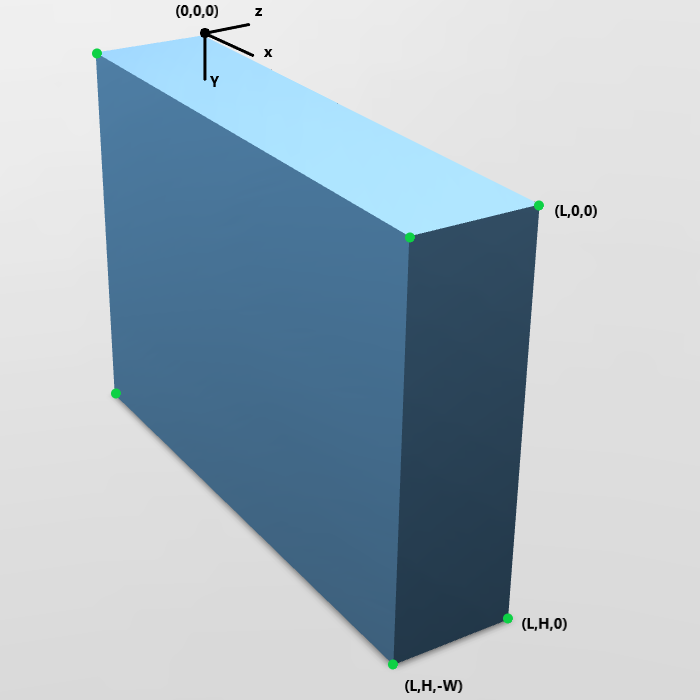
\includegraphics[width=0.75\textwidth]{BoxModel.png}
%		\caption{Rigid object model.} \label{box}
%	\end{minipage}\hfill
%	\begin{minipage}{0.5\textwidth}
%		\begin{center}
%			\begin{tabular}[5pt]{| c| c|}
%				\hline
%				Parameter	& Value (cm) \\[0.5ex] 
%				\hline 	
%				Length& 45.6  \\ \hline 
%				Height& 32.5  \\ \hline 
%				Width& 10.1  \\ \hline 
%			\end{tabular}
%			\captionof{table}{Object Dimensions}\label{boxdim}
%		\end{center}	
%	\end{minipage}
%\end{figure}


%	\begin{center}
%	\begin{tabular}[5pt]{| c| c|}
%		\hline
%		Point	& Angle(s) (degrees) \\[0.5ex] 
%		\hline 	
%		$1$& 103.6447 \\ \hline 
%		$2$& 82.6421, 90.4116  \\ \hline 
%		$3$& 88.9373  \\ \hline 
%		$4$& 91.496, 92.3435  \\ \hline 
%		$5$& 93.2852  \\ \hline 
%		$6$& 85.5876, 76.0264  \\ \hline 
%		$7$& 97.667, 88.7342, 89.1479  \\ \hline 
%	\end{tabular}
%	\captionof{table}{Object Dimensions}\label{angles}
%\end{center}	

\section{Conclusions}


\appendix % this command sets sectioning command to the appendix format
% uncomment the next line to start on a fresh page



\section{Code Listings}\label{code}

% input the file containing the code
%\lstinputlisting[caption={Top level implementation for Monocular Calibration and Pose Estimation},label={proj}]{MonoPose.m}
%\lstinputlisting[caption={QR Decomp Based Algorithm Implementation},label={alg}]{MonoPoseQR.m} 
%\lstinputlisting[caption={Rearranged QR Decomposition (Credit: Dr. John McInroy)},label={qrCom}]{qrCommute.m}


%% The commands below automatically generate the References section
%% using the ``sample_bib'' file I've given you.

%\newpage  % start a new page
%
%\bibliographystyle{ieeetr}
%\bibliography{a1_abbrv,Proj2}

\end{document} % always the last line of your document file
